% Options for packages loaded elsewhere
\PassOptionsToPackage{unicode}{hyperref}
\PassOptionsToPackage{hyphens}{url}
\PassOptionsToPackage{dvipsnames,svgnames,x11names}{xcolor}
%
\documentclass[
  authoryear]{elsarticle}

\usepackage{amsmath,amssymb}
\usepackage{iftex}
\ifPDFTeX
  \usepackage[T1]{fontenc}
  \usepackage[utf8]{inputenc}
  \usepackage{textcomp} % provide euro and other symbols
\else % if luatex or xetex
  \usepackage{unicode-math}
  \defaultfontfeatures{Scale=MatchLowercase}
  \defaultfontfeatures[\rmfamily]{Ligatures=TeX,Scale=1}
\fi
\usepackage{lmodern}
\ifPDFTeX\else  
    % xetex/luatex font selection
\fi
% Use upquote if available, for straight quotes in verbatim environments
\IfFileExists{upquote.sty}{\usepackage{upquote}}{}
\IfFileExists{microtype.sty}{% use microtype if available
  \usepackage[]{microtype}
  \UseMicrotypeSet[protrusion]{basicmath} % disable protrusion for tt fonts
}{}
\makeatletter
\@ifundefined{KOMAClassName}{% if non-KOMA class
  \IfFileExists{parskip.sty}{%
    \usepackage{parskip}
  }{% else
    \setlength{\parindent}{0pt}
    \setlength{\parskip}{6pt plus 2pt minus 1pt}}
}{% if KOMA class
  \KOMAoptions{parskip=half}}
\makeatother
\usepackage{xcolor}
\setlength{\emergencystretch}{3em} % prevent overfull lines
\setcounter{secnumdepth}{5}
% Make \paragraph and \subparagraph free-standing
\makeatletter
\ifx\paragraph\undefined\else
  \let\oldparagraph\paragraph
  \renewcommand{\paragraph}{
    \@ifstar
      \xxxParagraphStar
      \xxxParagraphNoStar
  }
  \newcommand{\xxxParagraphStar}[1]{\oldparagraph*{#1}\mbox{}}
  \newcommand{\xxxParagraphNoStar}[1]{\oldparagraph{#1}\mbox{}}
\fi
\ifx\subparagraph\undefined\else
  \let\oldsubparagraph\subparagraph
  \renewcommand{\subparagraph}{
    \@ifstar
      \xxxSubParagraphStar
      \xxxSubParagraphNoStar
  }
  \newcommand{\xxxSubParagraphStar}[1]{\oldsubparagraph*{#1}\mbox{}}
  \newcommand{\xxxSubParagraphNoStar}[1]{\oldsubparagraph{#1}\mbox{}}
\fi
\makeatother


\providecommand{\tightlist}{%
  \setlength{\itemsep}{0pt}\setlength{\parskip}{0pt}}\usepackage{longtable,booktabs,array}
\usepackage{calc} % for calculating minipage widths
% Correct order of tables after \paragraph or \subparagraph
\usepackage{etoolbox}
\makeatletter
\patchcmd\longtable{\par}{\if@noskipsec\mbox{}\fi\par}{}{}
\makeatother
% Allow footnotes in longtable head/foot
\IfFileExists{footnotehyper.sty}{\usepackage{footnotehyper}}{\usepackage{footnote}}
\makesavenoteenv{longtable}
\usepackage{graphicx}
\makeatletter
\newsavebox\pandoc@box
\newcommand*\pandocbounded[1]{% scales image to fit in text height/width
  \sbox\pandoc@box{#1}%
  \Gscale@div\@tempa{\textheight}{\dimexpr\ht\pandoc@box+\dp\pandoc@box\relax}%
  \Gscale@div\@tempb{\linewidth}{\wd\pandoc@box}%
  \ifdim\@tempb\p@<\@tempa\p@\let\@tempa\@tempb\fi% select the smaller of both
  \ifdim\@tempa\p@<\p@\scalebox{\@tempa}{\usebox\pandoc@box}%
  \else\usebox{\pandoc@box}%
  \fi%
}
% Set default figure placement to htbp
\def\fps@figure{htbp}
\makeatother

\usepackage{booktabs}
\usepackage{longtable}
\usepackage{array}
\usepackage{multirow}
\usepackage{wrapfig}
\usepackage{float}
\usepackage{colortbl}
\usepackage{pdflscape}
\usepackage{tabu}
\usepackage{threeparttable}
\usepackage{threeparttablex}
\usepackage[normalem]{ulem}
\usepackage{makecell}
\usepackage{xcolor}
\usepackage{graphicx}
\usepackage{adjustbox}
\makeatletter
\@ifpackageloaded{caption}{}{\usepackage{caption}}
\AtBeginDocument{%
\ifdefined\contentsname
  \renewcommand*\contentsname{Table of contents}
\else
  \newcommand\contentsname{Table of contents}
\fi
\ifdefined\listfigurename
  \renewcommand*\listfigurename{List of Figures}
\else
  \newcommand\listfigurename{List of Figures}
\fi
\ifdefined\listtablename
  \renewcommand*\listtablename{List of Tables}
\else
  \newcommand\listtablename{List of Tables}
\fi
\ifdefined\figurename
  \renewcommand*\figurename{Figure}
\else
  \newcommand\figurename{Figure}
\fi
\ifdefined\tablename
  \renewcommand*\tablename{Table}
\else
  \newcommand\tablename{Table}
\fi
}
\@ifpackageloaded{float}{}{\usepackage{float}}
\floatstyle{ruled}
\@ifundefined{c@chapter}{\newfloat{codelisting}{h}{lop}}{\newfloat{codelisting}{h}{lop}[chapter]}
\floatname{codelisting}{Listing}
\newcommand*\listoflistings{\listof{codelisting}{List of Listings}}
\makeatother
\makeatletter
\makeatother
\makeatletter
\@ifpackageloaded{caption}{}{\usepackage{caption}}
\@ifpackageloaded{subcaption}{}{\usepackage{subcaption}}
\makeatother
\journal{Financial Research Letters}

\usepackage[]{natbib}
\bibliographystyle{elsarticle-harv}
\usepackage{bookmark}

\IfFileExists{xurl.sty}{\usepackage{xurl}}{} % add URL line breaks if available
\urlstyle{same} % disable monospaced font for URLs
\hypersetup{
  pdftitle={A Stakeholder-Legitimacy Framework for ESG Disclosure in Banking Under Evolving Regulatory Mandates},
  pdfauthor={Ying (Veronica) Zhang; Lisa Sheenan; Fearghal Kearney; Junyu Zhang; Suma Mani; George Hutchinson; Neil Reid; Paul Brereton},
  pdfkeywords={ESG disclosure, IFRS S1 and S2, Stakeholder-Legitimacy
framework, bank risk, ownership, climate change},
  colorlinks=true,
  linkcolor={blue},
  filecolor={Maroon},
  citecolor={Blue},
  urlcolor={Blue},
  pdfcreator={LaTeX via pandoc}}


\setlength{\parindent}{6pt}
\begin{document}
\begin{frontmatter}
\title{A Stakeholder-Legitimacy Framework for ESG Disclosure in Banking
Under Evolving Regulatory Mandates \\\large{Literature Review of ESG
disclosure in Banking Industry} }

\author[1]{Ying (Veronica) Zhang%
\corref{cor1}%
}
 \ead{veronica.zhang@qub.ac.uk} 
\author[2]{Lisa Sheenan%
%
}
 \ead{lisa.sheenan@ucd.ie} 
\author[1]{Fearghal Kearney%
%
}
 \ead{f.kearney@qub.ac.uk} 
\author[3]{Junyu Zhang%
%
}

\author[3]{Suma Mani%
%
}

\author[3]{George Hutchinson%
%
}

\author[3]{Neil Reid%
%
}

\author[3]{Paul Brereton%
%
}

\affiliation[1]{organization={Queen's University, Belfast, Queen's
Business School},addressline={Belfast, UK},postcodesep={}}
\affiliation[2]{organization={University College Dublin, UCD College of
Business},addressline={Dublin, Ireland},postcodesep={}}
\affiliation[3]{organization={Queen's University, Belfast, School of
Biological Sciences},,postcodesep={}}

\cortext[cor1]{Corresponding author}








        
\begin{abstract}
The global financial sector is undergoing a transformative shift as
nature-related risks, from biodiversity loss to ecosystem degradation,
emerge as material threats to economic stability. By reviewing the
literature, this study advances a novel Stakeholder-Legitimacy
Framework, integrating stakeholder theory, legitimacy theory, and
institutional isomorphism to explain how banks' ESG disclosures emerge
from dynamic negotiations between external pressures (e.g., regulators,
investors) and strategic legitimacy-seeking behaviors. Key findings
reveal that while ESG disclosures mitigate bank-specific risks,
conflicting evidence persists on their financial performance impacts.
Critical gaps include underexplored transmission effects of regulations
through lending networks, inconsistent roles of institutional and state
ownership, and tensions between symbolic compliance and substantive
action.
\end{abstract}





\begin{keyword}
    ESG disclosure \sep IFRS S1 and S2 \sep Stakeholder-Legitimacy
framework \sep bank risk \sep ownership \sep 
    climate change
\end{keyword}
\end{frontmatter}
    

\section{Introduction}\label{introduction}

The global financial system is undergoing a seismic shift as
nature-related risks---ranging from biodiversity loss to ecosystem
degradation---emerge as material threats to economic stability
\citep{UNEP2023}. Over the past decade, voluntary sustainability
frameworks like the Task Force on Climate-related Financial Disclosures
(TCFD) have evolved into robust, jurisdictionally mandated systems,
driven by regulatory imperatives to combat greenwashing, harmonize
reporting standards, and align financial flows with planetary
boundaries. Central to this transformation are frameworks such as the
Task Force on Nature-Related Financial Disclosures (TNFD), the
International Sustainability Standards Board (ISSB), and region-specific
regulations like the EU's Corporate Sustainability Reporting Directive
(CSRD) and the UK's Sustainability Disclosure Requirements (SDR). These
frameworks reflect a growing consensus that environmental risks are
inextricably linked to financial performance, necessitating disclosures
that integrate double materiality---assessing both financial risks to
firms and firms' impacts on ecosystems.

Despite the systemic importance of banks, empirical research on how ESG
regulations affect their risk profiles, governance mechanisms, and
financial performance remains fragmented. Existing studies
disproportionately focus on non-financial firms
\citep[e.g.][]{YOUN2015, FAVINO2019, BUALLAY2019, DYCK2019}, leaving
critical gaps in understanding banks' unique intermediation role. For
instance, while the TNFD's LEAP methodology and the ISSB's IFRS S1 and
S2 standards are gaining traction, their sector-specific implications
for banking---such as transmission effects through lending networks or
the tension between symbolic compliance and substantive action---are
underexplored. Theoretical frameworks also remain fragmented, with
stakeholder theory, legitimacy theory, and institutional isomorphism
often treated in isolation rather than as interconnected drivers of ESG
disclosure. This review addresses these gaps by synthesizing global
evidence, proposing an integrated theoretical model, and identifying
urgent research priorities at the nexus of finance, regulation, and
ecological stewardship.

In this study, we advance a novel Stakeholder-Legitimacy Framework
\citep{CAMPBELL2007, AGUINIS2012} tailored to banks, synthesizing
stakeholder theory, legitimacy theory, and institutional isomorphism.
This model positions ESG disclosures as dynamic outcomes of external
pressures (e.g., regulators, shareholders) and banks' legitimacy-seeking
behaviors, moderated by economic factors (e.g., bank size) and
institutional contexts (e.g., ownership structures). We also find the
following critical research gaps:

\begin{itemize}
\item
  Ownership Dynamics: The role of institutional and state ownership in
  shaping ESG outcomes remains inconsistent across studies
  \citep{DYCK2019, RAIMO2020}, with concentrated ownership marginalizing
  minority shareholder influence on CSR practices \citep{SMITH2022}.
\item
  Regulatory Efficacy: Sector-specific analyses of mandatory frameworks
  (e.g., CSRD, EU Taxonomy) are scarce, particularly their impact on
  bank risk profiles and governance mechanisms.
\item
  Systemic Risk Implications: The interplay between ESG disclosures and
  systemic financial stability, especially during regulatory shocks
  (e.g., rapid green transitions), lacks empirical rigor
  \citep{ESRB2016}.
\end{itemize}

Our study contributes to sustainable finance research through three key
areas:

\begin{itemize}
\item
  Theoretical Innovation: The Stakeholder-Legitimacy Framework bridges
  siloed theories, offering a holistic lens to analyze banks' ESG
  disclosures as context-dependent processes shaped by stakeholder
  pressures and legitimacy imperatives.
\item
  Gap-Driven Agenda: By systematizing underexplored research gaps---such
  as regulatory transmission mechanisms and ownership dynamics---we
  provide a roadmap for future studies to address banking-specific
  complexities.
\item
  Policy Relevance: We identify actionable solutions for regulators,
  including integrating natural capital valuation into stress testing
  and harmonizing ISSB-TNFD interoperability to mitigate symbolic
  compliance risks.
\end{itemize}

The remainder of the literature review is organized as follows: Section
II provides an overview of the nature-related financial disclosure
frameworks from different dimensions. In Section III, we review the
theories underpinning the relationship between ESG disclosure and the
banking sector. In Section IV, we propose the integrated
Stakeholder-Legitimacy framework applied to the banking industry and
review the research gaps. Section V is the conclusion section.

\section{Overview of Nature-related Financial Disclosure
Frameworks}\label{overview-of-nature-related-financial-disclosure-frameworks}

\subsection{Evolution of Nature-Related Disclosure
Frameworks}\label{evolution-of-nature-related-disclosure-frameworks}

The global landscape of nature-related financial disclosures has
undergone a significant transformation over the past decade,
transitioning from fragmented voluntary initiatives to increasingly
robust, jurisdictionally mandated frameworks. This evolution reflects
growing recognition of nature-related risks as material to financial
stability, coupled with regulatory efforts to combat greenwashing and
harmonize reporting standards. Below, we outline key frameworks driving
this shift, with a focus on their progression toward mandatory adoption.

\subsubsection{Global Frameworks}\label{global-frameworks}

\begin{itemize}
\tightlist
\item
  \textbf{Task Force on Nature-Related Financial Disclosures (TNFD)}
\end{itemize}

Launched in June 2021 and finalized in September 2023, the TNFD builds
on the legacy of the Task Force on Climate-Related Financial Disclosures
(TCFD) by adapting its four-pillar structure --- governance, strategy,
risk and impact management, and metrics and targets --- to address
nature-specific risks. While the TCFD (2017) laid the groundwork for
voluntary climate disclosures, the TNFD expands this model to include
biodiversity loss, water security, and ecosystem degradation
\citep[see][]{TNFD2023}. The framework's alignment with the
Kunming-Montreal Global Biodiversity Framework (GBF) is codified in
Target 15, which requires corporations to ``monitor, assess, and
transparently disclose their risks, dependencies, and impacts on
biodiversity'' by 2030 \citep{CBD2023}. This positions the TNFD as a
critical tool for meeting international commitments.

While the TNFD remains voluntary, its design facilitates regulatory
adoption. For example, France's Energy and Climate Law (2023)\footnote{see
  \url{https://climate-laws.org/document/law-no-2023-973-of-october-23-2023-relating-to-the-green-industry_71cd}}
mandates TNFD-aligned reporting for financial institutions, citing the
framework's ``robust methodology for assessing portfolio exposure to
biodiversity risks''. Similarly, Brazil's Central Bank integrates TNFD
principles into its sustainability guidelines, emphasizing
``location-specific impacts on biomes such as the Amazon''
\citep{STUSSI2024}.

The TNFD Enhances the scope by adding 14 new disclosure recommendations
to the TCFD's original 11, emphasizing location-specific impacts, value
chain dependencies, and engagement with Indigenous communities. Its LEAP
approach (Locate, Evaluate, Assess, Prepare) provides a standardized
methodology for assessing nature-related risks, including for banks to
map portfolio exposures \citep[see][]{TNFD2023LEAP}.

\begin{itemize}
\tightlist
\item
  \textbf{ISSB Sustainability Disclosure Standards (IFRS S1 \& S2)}
\end{itemize}

The International Sustainability Standards Board (ISSB), established in
2021 at COP26, aims to unify global sustainability reporting through its
IFRS S1 (general sustainability disclosures) and IFRS S2
(climate-specific disclosures). IFRS S1 mandates that sustainability
disclosures be ``integrated into financial statements to ensure
comparability and reliability'' \citep{IFRS2023S1}, while IFRS S2
requires granular climate-related risk disclosures, including physical
and transition risks \citep{IFRS2023S2}. These standards consolidate the
TCFD's legacy into a mandatory global baseline, signaling a shift toward
mandatory, investor-grade disclosures.

The ISSB standards, endorsed by global organizations such as the G7,
G20, and IOSCO, are gaining rapid international adoption. Several
jurisdictions, including the UK, Japan, and Singapore, have already
announced plans to mandate alignment with IFRS S1 and S2 by 2025. For
instance, the UK government's 2023 policy paper confirms its intent to
adopt ISSB standards as the foundation for its UK Sustainability
Reporting Standards (UK SRS), with mandatory disclosures for listed
companies by 2025.\footnote{see
  \url{https://www.gov.uk/government/publications/sustainability-disclosure-requirements-implementation-update-2024}}

A key feature of these standards is their integration with financial
reporting. Unlike standalone ESG frameworks, IFRS S1 and S2 require
sustainability disclosures to be included within annual financial
statements, ensuring they are subject to the same level of scrutiny and
rigor as financial data. For banks, this means that nature-related
risks---such as loans linked to deforestation---must be disclosed
alongside traditional financial risks.

Additionally, the ISSB has collaborated with the Taskforce on
Nature-related Financial Disclosures (TNFD) to enhance interoperability.
This collaboration enables institutions to report both climate and
nature-related risks under a unified, compatible structure, simplifying
the reporting process while ensuring comprehensive risk assessment
\citep[see][]{TNFD2024}.

The alignment of IFRS S1 and S2 with relevant ESG disclosure frameworks
including TNFD is presented in Figure~\ref{fig-IFRS}.

\begin{figure}

\centering{

\pandocbounded{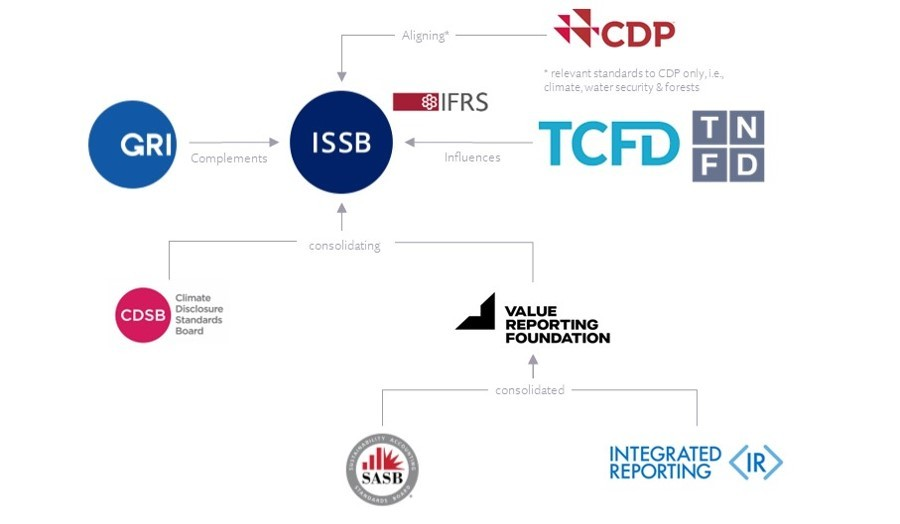
\includegraphics[keepaspectratio]{IFRS_S1S2.jpeg}}

}

\caption{\label{fig-IFRS}Alignment of IFRS S1 and S2}

\end{figure}%

\subsubsection{Regional Frameworks}\label{regional-frameworks}

\begin{itemize}
\tightlist
\item
  \textbf{European Union}
\end{itemize}

The EU has pioneered mandatory nature-related disclosures through three
interlinked regulations:

\begin{itemize}
\tightlist
\item
  \emph{EU Taxonomy Regulation (2020)}
\end{itemize}

The EU Taxonomy serves as a comprehensive classification system designed
to identify environmentally sustainable activities, incorporating strict
criteria for biodiversity protection and ecosystem
restoration\footnote{see
  \url{https://finance.ec.europa.eu/regulation-and-supervision/financial-services-legislation/implementing-and-delegated-acts/taxonomy-regulation_en}}.
It requires in-scope entities, including banks, to disclose
Taxonomy-aligned revenue, capital expenditures (CapEx), and operating
expenditures (OpEx). Failure to comply can result in reputational damage
and exclusion from sustainable finance markets, such as the EU green
bond market \citep{EBA2022}.

\begin{itemize}
\tightlist
\item
  \emph{Corporate Sustainability Reporting Directive (CSRD, 2023)}
\end{itemize}

The Corporate Sustainability Reporting Directive (CSRD) replaces the
voluntary Non-Financial Reporting Directive (NFRD), significantly
expanding its scope from 11,000 to over 50,000 EU and non-EU companies
by 2027. A cornerstone of the CSRD is its ``double materiality''
approach, which requires companies, including banks, to report on both
financial and impact-related risks. This includes the disclosure of
risks to ecosystems alongside traditional financial risks.

The CSRD introduces detailed reporting obligations under the European
Sustainability Reporting Standards (ESRS), including ESRS E4
(Biodiversity and Ecosystems). ESRS E4 mandates disclosures on several
key aspects:

\begin{itemize}
\tightlist
\item
  Dependencies: For example, the reliance on critical resources such as
  water for operations;
\item
  Impacts: Such as land degradation linked to lending portfolios;
\item
  Transition Plans: Strategies to mitigate nature-related risks.
\end{itemize}

Furthermore, ESRS E4 explicitly incorporates metrics from the Taskforce
on Nature-related Financial Disclosures (TNFD) for assessing impacts on
protected areas, ensuring alignment with established global frameworks
\citep[see][]{EFRAG2022}.

\begin{itemize}
\tightlist
\item
  \emph{Sustainable Finance Disclosure Regulation (SFDR, 2021)}
\end{itemize}

The Sustainable Finance Disclosure Regulation (SFDR) requires financial
institutions to classify investment products based on their
sustainability objectives under Articles 6, 8, or 9 and to disclose
their alignment with the EU Taxonomy.\footnote{see
  \url{https://finance.ec.europa.eu/sustainable-finance/disclosures/sustainability-related-disclosure-financial-services-sector_en}}

Under the Do No Significant Harm (DNSH) principle, banks are now
obligated to screen investments for activities that may harm
biodiversity, such as logging in protected areas. Furthermore, Article 9
of the SFDR mandates comprehensive due diligence to ensure investments
do not negatively impact biodiversity, emphasizing the importance of
sustainable investment practices.

\begin{itemize}
\tightlist
\item
  \textbf{United Kingdom}
\end{itemize}

The UK's Sustainability Disclosure Requirements (SDR) policy framework,
as outlined in HM Treasury's 2023 roadmap, integrates the ISSB standards
while mandating the inclusion of ``transition plans aligned with the
Paris Agreement and the Global Biodiversity Framework
(GBF).''\footnote{see
  \url{https://www.gov.uk/government/publications/sustainability-disclosure-requirements-implementation-update-2024}}

A key component of this framework is the development of the UK
Sustainability Reporting Standards (UK SRS), which are expected to be
finalized by 2025. These standards will adopt ISSB guidelines while
incorporating UK-specific requirements, such as transition planning
disclosures for high-emitting sectors.

Mandatory disclosures for listed companies will commence in 2026. Banks
will be required to report on financed emissions and nature-related risk
exposures, with a particular focus on high-impact sectors such as
agriculture and mining. The Financial Conduct Authority (FCA) will
enforce these disclosure requirements, ensuring compliance by banks
starting in 2026 \citep[see][]{FCA2023}.

The SDR explicitly references the recommendations of the Taskforce on
Nature-related Financial Disclosures (TNFD), ensuring consistency with
international biodiversity goals and strengthening its alignment with
global sustainability frameworks.

\begin{itemize}
\tightlist
\item
  \textbf{United States}
\end{itemize}

The U.S. Securities and Exchange Commission's (SEC) Climate Disclosure
Rule (2024) marks the country's first federal initiative to mandate
nature-related disclosures.\footnote{see
  \url{https://www.sec.gov/rules-regulations/2024/03/s7-10-22\#:~:text=The\%20final\%20rules\%20will\%20require,of\%20operations\%2C\%20or\%20financial\%20condition.}}
However, its implementation has been delayed due to ongoing legal
challenges.

The rule mandates that public companies disclose material climate risks,
such as physical risks from severe weather events (e.g., floods), along
with Scope 1, 2, and 3 greenhouse gas emissions. Additionally, companies
must report costs associated with extreme weather impacts.

While federal efforts face delays, California has taken significant
steps with the Climate Corporate Data Accountability Act (SB 253).
Effective in 2026, this law requires companies with annual revenues
exceeding \$1 billion to report Scope 1, 2, and 3 emissions. The
legislation emphasizes addressing systemic risks from biodiversity loss
within supply chains, indirectly pressuring banks and financial
institutions to assess the nature-related risks of their
clients.\footnote{see
  \url{https://leginfo.legislature.ca.gov/faces/billNavClient.xhtml?bill_id=202320240SB253\#:~:text=The\%20act\%20requires\%20the\%20state,the\%20state\%20board\%2C\%20as\%20provided.}}

The summary information of regional ESG regulatory frameworks can be
found in Table~\ref{tbl-regional}.

\begin{table}

\caption{\label{tbl-regional}Regional ESG Disclosure Regulations}

\centering{

\centering\begingroup\fontsize{11}{13}\selectfont

\resizebox{\ifdim\width>\linewidth\linewidth\else\width\fi}{!}{
\begin{tabular}[t]{>{\raggedright\arraybackslash}p{5em}>{\raggedright\arraybackslash}p{8em}>{\raggedleft\arraybackslash}p{5em}>{\raggedright\arraybackslash}p{12em}>{\raggedright\arraybackslash}p{8em}>{\raggedright\arraybackslash}p{10em}>{\raggedright\arraybackslash}p{10em}}
\toprule
\multicolumn{1}{c}{\cellcolor{lightgray}{\textbf{Region}}} & \multicolumn{1}{c}{\cellcolor{lightgray}{\textbf{Regulation}}} & \multicolumn{1}{c}{\cellcolor{lightgray}{\textbf{Year}}} & \multicolumn{1}{c}{\cellcolor{lightgray}{\textbf{Key\_features}}} & \multicolumn{1}{c}{\cellcolor{lightgray}{\textbf{Scope}}} & \multicolumn{1}{c}{\cellcolor{lightgray}{\textbf{Enforcement}}} & \multicolumn{1}{c}{\cellcolor{lightgray}{\textbf{Alignment}}}\\
\midrule
\cellcolor{gray!10}{EU} & \cellcolor{gray!10}{EU Taxonomy Regulation} & \cellcolor{gray!10}{2020} & \cellcolor{gray!10}{a comprehensiver classification system designed to identify environmentally sustainable activities} & \cellcolor{gray!10}{Banks and in-scope entities} & \cellcolor{gray!10}{Failure to comply can result in reputational damage and exclusion from sustainable finance markets} & \cellcolor{gray!10}{EU Taxonomy classification system}\\
EU & Corporate Sustainability Reporting Directive (CSRD) & 2023 & 'double materiality' approach; ESRS & 50,000+ EU/non-EU companies by 2027 & Mandatory for EU/non-EU companies & Aligns with IFRS S1 and S2 standards; TNFD metrics\\
\cellcolor{gray!10}{EU} & \cellcolor{gray!10}{Sustainable Finance Disclosure Regulation (SFDR)} & \cellcolor{gray!10}{2021} & \cellcolor{gray!10}{financial institutions classify investment products based on their sustainability objectives} & \cellcolor{gray!10}{Financial institutions} & \cellcolor{gray!10}{Market exclusion for non-compliance} & \cellcolor{gray!10}{Links to EU Taxonomy}\\
UK & Sustainability Disclosure Requirements (SDR) & 2023 & ISSB-aligned reporting; Transition plans for Paris and GBF; Financed emissions disclosure & Listed companies (from 2026); High-impact sectors (agriculture, mining) & FCA enforcement starting 2026 & Aligns with IFRS S1 and S2; References TNFD recommendations\\
\cellcolor{gray!10}{US} & \cellcolor{gray!10}{SEC Climate Disclosure Rule} & \cellcolor{gray!10}{2024} & \cellcolor{gray!10}{Material climate risk disclosure; Scope 1-3 emissions reporting; Extreme weather cost reporting} & \cellcolor{gray!10}{Public companies} & \cellcolor{gray!10}{Delayed due to legal challenges} & \cellcolor{gray!10}{N/A}\\
\addlinespace
US & Climate Corporate Data Accountability Act (SB 253) & 2026 & Scope 1-3 emissions reporting for \$1B+ revenue firms; Biodiversity risk assessment & Large corporations operating in California & California state law enforcement & Addresses supply chain biodiversity risks\\
\bottomrule
\end{tabular}}
\endgroup{}

}

\end{table}%

\subsubsection{From Voluntary to Mandatory: Key Drivers and
Challenges}\label{from-voluntary-to-mandatory-key-drivers-and-challenges}

The shift toward mandatory nature-related disclosure frameworks is
driven by several key developments, reflecting the growing recognition
of environmental risks and the need for harmonized reporting standards.

\begin{itemize}
\tightlist
\item
  \emph{Recognition of Material Nature-Related Risks}
\end{itemize}

Increasing awareness of biodiversity loss, ecosystem degradation, and
water security as critical threats to financial stability has
accelerated the move toward mandatory disclosures. Frameworks like the
Taskforce on Nature-related Financial Disclosures (TNFD) emphasize the
financial materiality of these risks to corporate and institutional
performance. The widespread adoption of the TNFD by over 320
institutions, including major banks and asset managers, underscores the
influence of investor demand for transparency and the need to assess
portfolio exposures to nature-related risks \citep{TNFD2023}.

\begin{itemize}
\tightlist
\item
  \emph{Global Regulatory Alignment}
\end{itemize}

The harmonization of sustainability reporting standards, led by
initiatives such as the ISSB's IFRS S1 and S2 and the TNFD, promotes
consistency and comparability across jurisdictions. These frameworks
explicitly reference global commitments like the Kunming-Montreal Global
Biodiversity Framework, solidifying their role in supporting
international biodiversity and sustainability goals.

\begin{itemize}
\tightlist
\item
  \emph{Integration with Financial Reporting}
\end{itemize}

Mandates under frameworks such as the ISSB standards \citep{IFRS2023S1}
and the EU's Corporate Sustainability Reporting Directive (CSRD) require
nature-related disclosures to be included in financial statements. This
integration enhances the rigor of sustainability reporting, ensuring it
is held to the same standards of accuracy and reliability as financial
data.

However, this transition also presents significant challenges that must
be addressed for effective implementation.

\begin{itemize}
\tightlist
\item
  \emph{Legal and Political Barriers}
\end{itemize}

Legal and political resistance has hindered the implementation of
mandatory disclosures in some jurisdictions. For example, the SEC's
Climate Disclosure Rule in the United States has faced significant legal
challenges, delaying its roll-out and highlighting the contentious
nature of regulatory enforcement in this domain.

\begin{itemize}
\tightlist
\item
  \emph{Complexity of Frameworks}
\end{itemize}

The proliferation of overlapping frameworks, including the TNFD, ISSB,
and various regional regulations, creates challenges for organizations,
particularly those operating in multiple jurisdictions. These entities
must navigate differing requirements, increasing the complexity and
administrative burden of compliance.

\begin{itemize}
\tightlist
\item
  \emph{Data Availability and Granularity}
\end{itemize}

Effective nature-related disclosure requires detailed and
location-specific data, such as ecosystem impacts and value chain
dependencies. Many organizations, especially those in sectors with
intricate supply chains, face difficulties in accessing or generating
the necessary data to meet disclosure requirements.

\section{ESG disclsoure and Banks}\label{esg-disclsoure-and-banks}

\subsection{Theoretical Foundation}\label{theoretical-foundation}

The relationship between environmental, social, and governance (ESG)
reporting and financial institutions has garnered increasing scholarly
attention, driven by global sustainability challenges. This section
synthesizes theoretical frameworks that explain how and why ESG
reporting influences financial institutions' operations,
decision-making, and market outcomes. Four interconnected theoretical
streams provide the foundation: organizational theories, economic
theories, institutional theory, and emerging frameworks such as natural
capital and double materiality.

\subsubsection{Organizational Theories}\label{organizational-theories}

Organizational theories, particularly stakeholder theory and legitimacy
theory, highlight the institutional motivations and external pressures
driving ESG reporting practices. Stakeholder theory, developed by
\citet{FREEMAN1984}, posits that organizations are accountable to a
broad range of stakeholders beyond shareholders, including regulators,
customers (investors), employees, and civil society. Building on this,
\citet{MITCHELL1997} proposed the theory of stakeholder salience
emphasizing understanding why and how managers prioritize certain
stakeholders, rather than prescribing whom they should prioritize. Their
theory provides tools to identify stakeholder types via a typology and
explain managerial responses through the concept of salience, which
assesses stakeholders' legitimacy, power, and urgency. This typology
offers a framework for financial institutions to navigate competing
stakeholder interests effectively. \citet{DONALDSON1995} provided
theoretical justification for stakeholder theory, emphasizing its
descriptive, instrumental, and normative validity in explaining
corporate behavior. \citet{ROBERTS1992} conducts an application of
stakeholder theory to explain corporate social responsibility
disclosure. The study finds that measures of stakeholder power,
strategic posture, and economic performance are significantly associated
with levels of corporate social disclosure. Banks' ESG disclosure, for
instance, on climate risks or green lending portfolios are often framed
as responses to investor demands for transparency or regulatory mandates
like the EU's Corporate Sustainability Reporting Directive (CSRD).

Legitimacy theory, foundationally developed by \citet{SUCHMAN1995},
identifies three primary forms of legitimacy\footnote{Legitimacy is a
  generalized perception or assumption that the actions of an entity are
  desirable, proper, or appropriate within some socially constructed
  system of norms, values, beliefs, and definitions
  \citep{GINZEL2004, NEILSEN1987, PERROW1970}.}---pragmatic, moral, and
cognitive---that organizations seek to maintain. \citet{DEEGAN2002}
applied this framework to environmental and social disclosures,
demonstrating how these practices reinforce an organization's
legitimacy. Firms' legitimacy-seeking behaviors influence the depth and
scope of disclosures, with firms in environmentally sensitive industries
disclosing more to manage public perception.

In the context of financial institutions, empirical studies show that
ESG reporting is often used to satisfy stakeholder demands and enhance
legitimacy. \citet{THOMPSON2004} examines how banks respond to
environmental stakeholders through reporting practices. Their findings
reveal that bankers value annual reports for assessing corporate
environmental impact, despite their limitations, and express some
interest in expanded environmental disclosures. However, their focus
primarily aims at safeguarding loans. Similarly, \citet{SCHOLTENS2009}
analyze how international banks balance different stakeholder interests
through Corporate Social Responsibility (CSR) reporting, while
\citet{CARNEVALE2014} test the direct effects of the sustainability
report on stock price in European markets, demonstrating that
sustainability reports positively influence stock prices by signaling
organizational compliance with evolving norms. \citet{MURE2021} provide
empirical evidence supporting stakeholder theory and legitimacy theory
that ESG disclosure and performance can be used by banks as a tool to
manage their reputation and maintain stakeholder trust, especially in
the face of adverse events.

\subsubsection{Economic Theories}\label{economic-theories}

Economic theories, particularly information asymmetry and agency theory,
explain how ESG reporting enhances market efficiency and reduces capital
costs. \citet{JENSEN1976} established the foundational agency theory
framework, explaining the conflicts of interest between principals
(shareholders) and agents (managers). This study lays the groundwork for
understanding how ESG reporting can mitigate agency costs by aligning
stakeholder interests. \citet{AKERLOF1970} work on Information Asymmetry
further explains how unequal information among market participants
creates inefficiencies. \citet{HART1987} provide a foundation for modern
contract theory and influence the theory of the firm and organizational
economics. This paper develops the principal-agent model, and
demonstrate how disclosure requirements can act as screening devices.
\citet{GRAY1996} provide a theoretical framework for understanding the
role of corporate social and environmental reporting in addressing
information asymmetry and enhancing accountability. Applying these
theories, studies have demonstrated that ESG disclosure reduces
information gaps and lowers agency costs, thereby enhancing market
efficiency. For instance, \citet{DHALIWAL2011} and \citet{ELGHOUL2011}
find firms that initiate CSR disclosure and have superior CSR
performance (relative to their industry peers) experience a subsequent
reduction in their cost of equity capital, and attract more dedicated
institutional investors and analyst coverage. Moreover, \citet{CUI2018}
observed that CSR engagement is inversely associated with reputation
risk, largely due to reduced information asymmetry.

\subsubsection{Institutional Isomorphism
Framework}\label{institutional-isomorphism-framework}

Institutional isomorphism framework explains the standardization and
diffusion of reporting practices. \citet{DIMAGGIO1983} identify three
mechanisms driving institutional isomorphism: Coercive isomorphism,
Mimetic isomorphism and Normative isomorphism. Their foundation study
develops a theoretical framework explaining how these mechanisms operate
within organizational fields - recognized areas of institutional life
where organizations interact under similar pressures. This framework is
valuable in understanding the standardization and diffusion of reporting
practices across organizations. Coercive isomorphism explains how
regulatory requirements and pressure from stakeholders drive adoption of
standardized reporting formats. Mimetic isomorphism illuminates why
organizations copy ``best practice'' reporting methods from industry
leaders during periods of uncertainty. Normative isomorphism shows how
professional networks and training lead to similar reporting approaches
across organizations. Empirical research highlights the importance of
institutional pressures, including coercive, normative, and mimetic
forces, in driving firms to conform to ESG expectations
\citep{DELMAS2004, HIGGINS2014, BEBBINGTON2018, CHRISTENSEN2021}.

\subsubsection{Emerging Theoretical
Concepts}\label{emerging-theoretical-concepts}

Emerging theoretical concepts and analytical lenses around natural
capital and double materiality offer novel perspectives on integrating
environmental considerations into financial decision-making. Natural
capital concept, as articulated by \citet{DASGUPTA2021} and
\citet{DAILY2009}, emphasizes the valuation of biodiversity and natural
capital, with implications for financial modeling \citep{ATKINSON2014}.
\citet{ECCLES2014} provide a theoretical foundation for integrated
reporting, which aligns closely with double materiality. The concept of
``double-materiality'' was first formally proposed by the European
Commission \citep{EC2019} in Guidelines on Non-financial Reporting:
Supplement on Reporting Climate-related Information published in June
2019; then was formalized by the regulation of the Corporate
Sustainability Reporting Directive (CSRD)\citep[see][]{EU_CSRD_2022} as
a reporting requirement. It mandates a company to judge materiality from
two perspectives 1) ``the extent necessary for an understanding of the
company's development, performance and position'' and ``in the broad
sense of affecting the value of the company''; 2) environmental and
social impact of the company's activities on a broad range of
stakeholders.

ESG disclosure and reporting has a positive influence on a company's
financial performance and risk. ESG reporting is not merely a compliance
exercise but a strategic imperative for financial institutions.

\subsection{Empirical Research}\label{empirical-research}

\subsubsection{Firm Value and
Performance}\label{firm-value-and-performance}

Stakeholder theories \citep[see][]{FREEMAN1984, DEEGAN2002} suggest that
when organizations incorporate environmental, social, and governance
(ESG) practices into their long-term strategic planning, they gain
competitive advantages by addressing the needs of various groups - from
employees and customers to government bodies and community members. This
approach recognizes that business success is linked to creating value
for all stakeholders, not just shareholders. In contrast, the trade-off
hypothesis or traditionalist view \citep[see][]{FRIEDMAN2007} suggests
ESG practices negatively impact financial performance by increasing
costs, harming corporate performance, and reducing competitive
advantage. Scholars argue that focusing on social and environmental
goals diverts managers from maximizing shareholder value. Similarly,
satisfying non-shareholder stakeholders may hinder profit maximization
and value creation for owners and managers\citep{GALANT2017}.

Empirical studies on the relationship between ESG engagement and
financial performance have provided conflicting findings. Driven by
stakeholder theory, \citet{WU2013} find that ESG disclosures improve
bank profitability by attracting ESG-conscious investors. Their findings
attribute to stakeholder pressure for transparency. Drawing from
empirical analysis using MSCI ESG STATS database ratings,
\citet{CORNETT2016} examine the relationship between the US commercial
banks' corporate social responsibility (CSR) practices and financial
performance. The study reveals that larger banks, despite facing
criticism for profit-focused practices leading to the crisis,
demonstrate consistently higher CSR strengths and concerns. Post-2009,
these institutions showed marked improvement with increased CSR
strengths and decreased concerns. Similarly, studies such as
\citet{CARNEVALE2014}, \citet{SHEN2016} and \citet{BUALLAY2021}
demonstrate bank's engagement in CSR activities can improve the
financial performance. While \citet{FERRERO2016} find a nonlinear
relationship between ESG and financial performance employing listed
companies in Europe. Moreover, \citet{BUALLAY2023} investigate the
effect of sustainability reporting on bank's performance (operational,
financial and market) in 7 regions that include 60 countries over the
period 2008--2017. They find the negative relationship between ESG
disclosures and banks' operational performance (ROA, ROE), and market
performance (Tobin's Q). They argue that sustainability reporting may
have negative impact on banks' asset utilization, in line with the
trad-off theory \citep[see][]{LEE2009}.

\subsubsection{Bank Risk}\label{bank-risk}

Despite growing scholarly attention to the link between CSR and bank
performance, empirical research examining its influence on risk exposure
within financial institutions remains limited. The existing literature
primarily focuses on individual bank risk metrics. A study by
\citet{GANGI2019} examine 142 banks across 35 countries and find that
stronger environmental engagement correlates with lower risk profiles as
measured by Z-scores \citep[see][]{LAEVEN2009}. Similarly,
\citet{SCHOLTENS2019} report a modest negative relationship between
sustainability practices and standalone risk measures among European
banks. Aligning with stakeholder theory, \citet{DI_TOMMASO2020}
demonstrate that higher ESG scores slightly curbed risk-taking among
European banks (2007--2018), though this relationship was mediated by
board composition factors including size, independent director presence,
and gender diversity. \citet{GANGWANI2024} report that higher ESG
disclosure scores correlate with reduced commercial banking risks,
specifically mitigating insolvency, leverage, and liquidity challenges.
Further evidence from \citet{CHIARAMONTE2022} demonstrate that both
aggregate ESG scores and individual pillars enhanced bank stability
during financial stress periods, with longer ESG disclosure histories
amplifying these stabilizing effects. Expanding geographically,
\citet{NEITZERT2022} examine 582 international banks (2002--2018),
corroborating the risk-mitigating effects of CSR activities on default
and portfolio risks, consistent with risk management frameworks.
However, their findings revealed heterogeneity across ESG pillars:
environmental (E) initiatives exhibited the strongest and most
consistent risk-reduction outcomes, whereas social (S) and governance
(G) dimensions yielded less definitive results.

Academic research on the relationship between systemic financial risk
and ESG factors remains limited, with existing studies examining each of
the three E, S and G pillars respectively. Regarding environmental (E)
factors, \citet{ESRB2016} points that an unanticipated rapid green
transition could significantly impact asset values, with
carbon-intensive investments facing declining profitability while
low-carbon assets appreciate. In terms of governance (G) factors,
\citet{ANGINER2018} present compelling evidence that
shareholder-friendly corporate governance structures correlate with
increased bank systemic risk, as measured by Marginal Expected Shortfall
(MES)\citep{ACHARYA2017} and SRISK metrics \citep{BROWNLEES2017}.This
relationship appears particularly pronounced for larger banks,
potentially due to too-big-to-fail considerations, and is amplified in
jurisdictions with more generous financial safety nets. Their findings
derive from analyses of both U.S. banks (1990-2014) and international
banks (2004-2008), suggesting the robustness of this relationship across
different contexts and time periods.

Using qualitative research method, \citet{KUHN2022} investigates
sustainable finance disclosures and initiatives in Germany. They find
that ESG disclosures enable financial institutions to identify exposure
to sectors with high dependency on vulnerable ecosystems. Disclosing
these dependencies improves transparency and helps institutions avoid
investments in activities contributing to ecological degradation such as
deforestation-linked loans. Their study proposes integrating natural
capital valuation into credit risk assessments to account for ``hidden''
risks. Case studies demonstrate that institutions adopting such
frameworks reduce exposure to stranded assets and regulatory penalties.

\subsubsection{Investment Strategy and Portfolio
Alignment}\label{investment-strategy-and-portfolio-alignment}

Banks have revised their approach to corporate social responsibility
(CSR), placing greater emphasis on managing both direct and indirect
risks associated with lending to firms facing environmental and social
challenges \citep{CARNEVALE2012}. Drawn on the stakeholder theory,
\citet{GOSS2011} examine the link between CSR and the cost of bank
loans. They find that firms with poor CSR performance face higher loan
costs due to the creditor risk perceptions.

\citet{DEMETRIADES2025} investigate lending patterns between major banks
and fossil fuel companies from 2001-2021 using global syndicated loan
data. They find a complex dynamic where banks recognize and price in
climate risks through higher interest rates and shorter loan terms, yet
simultaneously increase loan volumes to brown firms. The findings
suggest that regulatory pressure, particularly in Europe and the US, has
led to more stringent lending policies, though not necessarily reduced
lending volumes.

\citet{BASU2022} report that high-ESG banks complement, rather than
substitute, mortgage lending with community development investments in
poor areas. However, banks are more likely to reject mortgage
applications from these communities, suggesting social washing---using
pro-social rhetoric while limiting actual support. Their findings align
with the legitimacy theory, as banks appear to engage in CSR initiatives
to maintain societal approval rather than genuinely addressing financial
inclusion and social responsibility.

\subsubsection{Double Materiality}\label{double-materiality}

\citet{ARAS2024} investigates the SDGs with ESG indicators through a
double materiality perspective for 1888 companies from the OECD
financial institutions. The study shows how commercial banks can
identify and prioritize the SDGs and targets and how sustainable
practices at the corporate level can contribute to achieving these
global goals by adopting a sound approach.

\subsection{Research Gap and Proposed
Framework}\label{research-gap-and-proposed-framework}

In the early 2000s, \citet{HOOGHIEMSTRA2000} argues that sustainability
reporting research exhibits diverse and inconsistent findings, primarily
due to the absence of a comprehensive theoretical framework. The
research asserts that legitimacy was the dominant perspective.
\citet{SPENCE2010} identified stakeholder theory as the predominant and
most effective framework for explaining sustainability reporting
practices. They also point out that while many studies mention
stakeholders in general, they do not explicitly reference stakeholder
theory or other theoretical frameworks. Our review confirms their
observations in the literature of banks' ESG disclosure. The majority of
the studies show a preoccupation with stakeholder theory
\citep{GALANT2017, SHEN2016, BUALLAY2021}, legitimacy theory
\citep[e.g.][]{CARNEVALE2014}, and to some extent also institutional
theory \citep{HIGGINS2014, BEBBINGTON2018, CHRISTENSEN2021}. Moreover,
these studies primarily rely on isolated theoretical frameworks rather
than adopting a more holistic approach that integrates multiple
theoretical perspectives on ESG disclosure. In this review we propose an
integrated Stakeholder-Legitimacy Framework of banks' ESG disclosure,
which synthesizes and extends insights from \citet{CAMPBELL2007}
institutional-economic model and \citet{AGUINIS2012} multilevel CSR
analysis. At its core, the framework positions ESG disclosures as
outcomes of dynamic negotiations between stakeholder pressures and
legitimacy-seeking behaviors, moderated by banks' economic and
institutional contexts.

\begin{figure}

\centering{

\pandocbounded{\includegraphics[keepaspectratio]{flowchart.pdf}}

}

\caption{\label{fig-flowchart}ESG Disclosure Flowchart}

\end{figure}%

In the integrated framework (Figure~\ref{fig-flowchart}), stakeholder
pressures act as catalysts for banks' ESG disclosures. According to
stakeholder theory, companies should consider and balance the diverse
viewpoints and expectations of all groups affected by or invested in
their operations, rather than focusing solely on shareholders
\citep{BUCHHOLZ2005, LAPLUME2008}. \citet{FREEMAN1984} suggests that
company management should stay attuned to changing dynamics and trends
affecting both their organization's internal constituents and outside
parties. Stakeholder pressures arise from key external actors, including
regulators, investors, and customers. These actors demand greater
transparency and accountability, motivating banks to provide valuable
explanations of how they answer to the societal call for sustainable
business conduct. Banks respond to these pressures through strategic
legitimacy-seeking behaviors. Banks' ESG disclosures range from symbolic
gestures (e.g.~adopting TCFD guidelines without operational changes) to
substantive actions such as phasing out coal financing. Crucially,
legitimacy is not a static achievement but an ongoing process; banks
must continuously adapt to shifting norms, such as the rise of the TNFD
as a biodiversity benchmark. In the stakeholder-legitimacy context,
influential stakeholders execute greater pressure on companies to
explain and justify their business conduct. Therefore, sustainable
reporting and disclosed ESG information serve as a way for companies to
establish and maintain their legitimacy in the eyes of these
stakeholders \citep{CAMPBELL_D2003}.

The integrated framework further incorporates moderating contexts that
shape ESG disclosures produced by the translation of stakeholder
pressures into banks' legitimacy-seeking behaviors, including economic
conditions such as size and profitability, and institutional context
such as ownership structure and regulatory regimes.

\subsubsection{Bank Size and Financial
Perfromance}\label{bank-size-and-financial-perfromance}

Firm size (usually measured by total assets or market capitalization)
can be considered to have a positive effect on the adoption and extent
of ESG disclosure. As ESG engagements involve complex processes and
require a large scale to be effective \citep{YOUN2015}, firm size is a
critical factor in making them successful. Furthermore, according to
academic research, company visibility plays a crucial role in engaging a
broader and more heterogeneous set of stakeholders \citep{PELOZA2006}.
Visibility encourages organizations to adhere to social pressures and to
be more sensitive to stakeholders' expectations. And firm size is
positively associated with company visability \citep{MEZNAR1995}.
Therefore, companies with significant market visibility tend to
prioritize enhanced sustainability initiatives, motivated by the desire
to maintain a positive reputation among their stakeholders
\citep{DAMATO2020, ABDI2022}. The empirical studies of
\citet{FAVINO2019} and \citet{ALAREENI2020} support this viewpoint. They
conclude that firm size is an important determinant of ESG scores, as
larger firms have more available resources to provide ESG data and are
more likely to have their ESG data available. \citet{DREMPETIC2020} find
that larger firms tend to have higher ESG scores compared to smaller
firms. They also argue that size bias in ESG ratings practice, with
larger firms receiving systematically better ESG evaluations.
\citet{BUALLAY2019} and \citet{LAMANDA2024} find consistent empirical
results in banking sector.

A body of literature study the relation between ESG
disclosure/performance and financial performance, mostly focusing on the
impact of ESG activities on financial performance
\citep{FAVINO2019, BUALLAY2019, DAMATO2020, ABDI2022, LAMANDA2024}.
Financial performance as a determinant of ESG disclosure receives less
academic attention. Due to their higher ability and flexibility of
handling the costs of disclosing, companies with higher profitability
(lower leverage and gearing) are often presumed by researchers to be
better positioned to cope with any negative impacts that might arise
from revealing unfavorable information in their ESG disclosure. However,
the empirical results are mixed. \citet{BRAMMER2008} report that firms
with higher leverage are less likely to make voluntary environmental
disclosures due to financial constraints and costs. The positive
relationship between profitability (measured by return on assets (ROA),
or return on equity (ROE)) are reported by \citet{HADDOCK2005},
\citet{LIU2009} and \citet{GAMERSCHLAG2011}. Their studies argue that
profitable companies are more likely to disclose ESG information as they
have more resources available to absorb the associated costs. While
\citet{DYDUCH2017} do not find a significant relationship between
financial performance and sustainability reporting in Polish listed
companies. \citet{YUEN2022} report a U-shaped relationship between ESG
activities and bank profitability.

\subsubsection{Ownership and Regulation}\label{ownership-and-regulation}

Ownership structure and regulation can be considered as external
influential factors that are beyond management control. Studies
examining different ownership variables have emerged primarily in recent
years. The most investigated ownership structure include a company's
listing status (publicly listed), institutional shareholding, government
involvement (state-owned), and shareholding concentration.

Publicly listed companies, in order to comply with regulations and to be
aligned with industry best practices, as well as to stay attuned to
stakeholder pressure and see societal legitimacy, tend to be actively
engaged in ESG reporting. \citet{HADDOCK2005} reports that public
offering is linked to greater adoption of social reporting practices.
Additionally, publicly listed companies tend to disclose more
sustainability-related information \citep{GAMERSCHLAG2011}. The publicly
listed ownership structure was primarily examined as a variable in
studies conducted before 2015. However, around 2020, publicly listed
companies were more commonly used as data samples rather than as a
subject of ownership structure analysis
\citep[e.g.][]{SAHASRANAMAM2020, AMEEN2022, ALOBAID2024}. In more recent
research, institutional shareholding has emerged as a key variable of
interest, such as \citet{DYCK2019}, \citet{CHEN2020}, and
\citet{AMEEN2022}. Institutional investors are defined as pension funds,
insurance companies, banks, sovereign wealth funds, and other
institutions that manage and invest funds on behalf of their
beneficiaries; they are major players in the global financial markets
\citep{AMEEN2022}. Aligned with agency theory, \citet{SHLEIFER1986}
posit that institutional investors, leveraging their significant equity
stakes and specialized expertise, closely monitor corporate operations.
This oversight helps mitigate agency costs by ensuring management
decisions align with shareholder priorities, ultimately promoting more
efficient investment practices such as facilitating takeovers. Due to
their influential position, institutional investors can shape companies'
ESG initiatives by execute the stakeholder pressure on management to
disclose greater ESG-related data, aiming to fulfill non-financial goals
and bolster both their own and the firms' public image
\citep{DYCK2019, GARCIA-SANCHEZ2020}. Nevertheless, empirical literature
provides inconsistent findings. Some studies indicate that there is a
positive association between institutional ownership and ESG performance
\citep{DYCK2019, CHEN2020, AMEEN2022, RAIMO2020}. \citet{ZHOU2019}
repots that higher institutional ownership can facilitate firms'
transparency by providing voluntary CSR reports. \citet{ALUCHNA2022}
find a negative association between institutional ownership and
disclosure of the social performance. \citet{QU2007} produces
insignificant results on the relationship between corporate ownership,
including institutional ownership and state ownership, and a company's
CSR engagement.

While institutional investors' role in ESG practices has garnered
significant attention, the influence of state ownership introduces
distinct dynamics, particularly in balancing public policy objectives
with corporate accountability and transparency. \citet{TAGESSON2009}
find that State-owned corporations disclose more social information than
privately owned corporations. One explanation is that state-owned
corporations face heightened scrutiny, with pressure from their
government stakeholders and public/media attention driving demands for
accountability. These entities appear to have responded by aligning with
stakeholder demands, reflecting compliance with external expectations.
This fiding is also aligned with the social view of state ownership
theory \citep[see][]{STIGLITZ1993} that state ownership addresses market
failures and improve social welfare. \citet{LAU2016} and
\citet{ZHOU2019} support the social view that state ownership has a
significant positive impact on firms' CSR disclosure decisions.
\citet{BOSE2018} demonstrate that higher institutional ownership leads
to higher green banking disclosure. However, \citet{RAIMO2020} report a
negative relationship between state ownership and integrated report
quality. Shareholding concentration can mean that one or several
shareholders have substantial minority ownership stakes and voting
rights, such as 10 or 20 percent \citep{SHLEIFER1997}. Corporate
governance literature highlights the frequent comprimise of minority
shareholder rights in firms dominant controlling shareholders, where
concentrated ownership can lead to power imbalances and disproportionate
influence over strategic decisions \citep{SMITH2022}. Therefore,
\citet{SMITH2022} demonstrate that controlling shareholders are less
motivated to provide CSR information, with minority shareholders have
less power in CSR disclosure practices. \citet{BORGES2024} report that
large sharehoders have low interest in the firm's CSR reporting. This
result corroborates the finding by \citet{DUCASSY2015} that dominant
shareholders lack incentives to allocate resources to social initiatives
in contexts with limited stakeholder pressures to legitimize corporate
operations, which aligns with stakeholder theory and legitimacy theory.
\citet{LAU2016} also report that higher ownership concentration
negatively affects CSR performance.

Studies that exmaine the influence of ESG regulations are still scarce.
\citet{HESS2007} suggests that current vulantary initialtives of social
reporting are insufficienct to achieve coporate accountability. The
study argues, aligned with ligitamacy theory, that social reporting is
often driven by strategic considerations rather than a genuine
commitment to accountability. Companies may engage in social reporting
as a form of ``impression management'' to portray a positive image,
rather than to provide meaningful and transparent information to
stakeholders. \citet{HESS_etal2007} suggest that an overarching
mendatory social reporting system as the appropriate reporting system to
avoid corporate strategic disclosing behavior. \citet{QU2007} argues
that the robustness and enforcement of government regulations critically
shape the scope and depth of corporate social responsibility (CSR)
initiatives, underscoring regulatory frameworks as a catalyst in
advancing CSR practices by institutionalizing corporate accountability
and alignment with societal expectations. \citet{DESAI2024} reports that
stock market investors reacts positively to the mandatory ESG disclosure
regulation because mandatory ESG disclosure is considered as a positive
signal by reducing information asymmetry. \citet{KRUEGER2024}
demonstrate that mandatroy ESG disclosure improve firms' liquidity,
mitigating adverse selection problem. They also observe improvements in
liquidity as markets anticipate the introduction of mandatory ESG
disclosure regulations, reflecting proactive adjustments to expected
regulatory changes. \citet{LEE2024} find that compulsory ESG disclosure
regulation signifies the negative impact of ESG scores on firms' extreme
risks; the effect is amplified in cases where firms issue green bonds.
\citet{CICCHIELLO2023} examine the effects of NFRD. They argue that
government-mandated ESG disclosure regulations targeting corporate
social and environmental impacts are proven to strengthen both the rigor
and reliability of corporate disclosure practices, fostering greater
societal accountability. \citet{BOSE2018} demonstate that green banking
regulatory framework has positive association with green banking
disclosure practices. However, \citet{MANOS2024} report that
self-regulated banks have higher ESG scores by adopting Principles for
Responsible Banking (PRB). Additionally, their findings reveal the
negative impact of regulatory quality on ESG disclosure performance.
They argue that banks use mandatory ESG disclosure as a leverage to seek
ligitimacy in weaker institutional environment.

This section presents an integrated Stakeholder-Legitimacy Framework,
tailored to the banking sector, to explain banks' ESG disclosure
practices, synthesizing stakeholder theory, legitimacy theory, and
institutional contexts into a cohesive analytical pathway. The framework
posits that ESG disclosures arise from dynamic interactions between
external stakeholder pressures (e.g., regulators, investors, customers)
and banks' legitimacy-seeking behaviors, moderated by economic factors
(e.g., size, profitability) and institutional conditions (e.g.,
ownership structure, regulatory regimes). By bridging insights from
\citet{CAMPBELL2007} and \citet{AGUINIS2012}, the framework advances a
holistic view of ESG reporting as a negotiated outcome of strategic
adaptation to stakeholder demands and institutional expectations.

Critical research gaps persist, however. First, while institutional and
state ownership structures are increasingly scrutinized, findings remain
inconsistent: institutional ownership's role in ESG performance varies
across studies \citep[e.g.,][]{DYCK2019, ALUCHNA2022}, and state
ownership's dual mandate for social welfare and corporate accountability
lacks consensus \citep{TAGESSON2009, RAIMO2020}. Second, the moderating
role of regulatory frameworks is underexplored, particularly in the
highly regulated banking sector. Empirical research on how mandatory ESG
regulations (e.g., CSRD, EU Taxonomy) shape bank risk profiles,
financial performance, and governance mechanisms remains scarce, despite
the systemic importance of banks and their unique exposure to
ESG-related risks. While studies have begun analyzing disclosure quality
versus symbolic compliance in non-financial sectors
\citep{CICCHIELLO2023, MANOS2024}, sector-specific analyses for
banking---where regulatory pressures intersect with complex risk
intermediation roles---are urgently needed. Third, compounding this
complexity, banks' dual role in ESG ecosystems warrants deeper scrutiny:
as both reporting entities subject to disclosure mandates and financing
intermediaries influencing firms' access to green capital, they create
transmission effects that amplify regulatory impacts across economies.
For instance, \citet{WANG2023} demonstrates that ESG disclosure
regulations propagate through bank lending networks, altering borrowers'
environmental practices even without direct regulatory coverage---a
phenomenon underexplored in the literature. Fourth, mixed evidence on
the relationship between financial performance and ESG disclosure---such
as conflicting results on profitability
\citep{HADDOCK2005, DYDUCH2017}---highlights the need for contextualized
analyses. Finally, concentrated ownership's tendency to marginalize
minority shareholder influence on CSR practices
\citep{SMITH2022, BORGES2024} underscores a governance gap in aligning
dominant shareholders with broader stakeholder expectations. These gaps
signal opportunities for future research to refine the framework,
particularly in disentangling ownership dynamics, regulatory efficacy,
and the interplay between symbolic and substantive ESG strategies across
diverse institutional settings.

\section{Conclusion}\label{conclusion}

The transition from voluntary ESG initiatives to mandatory disclosure
frameworks marks a paradigm shift in how financial institutions
conceptualize and manage nature-related risks. Global frameworks like
the TNFD and ISSB, alongside regional regulations such as the EU
Taxonomy and CSRD, have established rigorous reporting standards that
integrate environmental impacts into financial decision-making. For
banks, these mandates necessitate not only transparency about their own
operations but also heightened scrutiny of borrowers' sustainability
practices \citep[see][]{WANG2023}, creating cascading effects across
economies. Empirical evidence suggests that ESG disclosures can mitigate
bank-specific risks---such as insolvency and liquidity
challenges---while improving market efficiency through reduced
information asymmetry \citep{GANGI2019, SCHOLTENS2019, GANGWANI2024}.
However, conflicting findings on the financial performance-ESG
relationship and the role of ownership structures underscore the need
for contextualized analyses.

To address these complexities, this review advances the
Stakeholder-Legitimacy Framework and tailor it to the banking sector.
This framework synthesizes stakeholder theory, legitimacy theory, and
institutional isomorphism to explain how banks' ESG disclosures emerge
from dynamic negotiations between external pressures (e.g., regulators,
investors) and legitimacy-seeking behaviors. It posits that banks
balance competing stakeholder demands---such as investor calls for
transparency and regulatory mandates for biodiversity due
diligence---through strategic disclosures that range from symbolic
compliance (e.g., superficial TNFD adoption) to substantive action
(e.g., divesting from deforestation-linked assets). Crucially, the
framework incorporates moderating factors such as ownership structures
(e.g., institutional ownership, state ownership) and regulatory regimes
(e.g., mandatory CSRD, vuluntary IFRS S1 and S2 adoption), offering a
nuanced lens to analyze how economic and institutional contexts shape
disclosure outcomes \citep{CAMPBELL2007, AGUINIS2012}.

Critical research gaps persist. First, the inconsistent role of
institutional and state ownership in shaping ESG outcomes highlights the
need for granular studies on how governance models mediate regulatory
compliance. Second, the banking sector's dual role as both reporting
entities and financial intermediaries remains underexplored,
particularly in how disclosure mandates transmit through lending
networks to influence unregulated firms. Third, the interplay between
symbolic compliance (e.g., adopting TNFD guidelines superficially) and
substantive action (e.g., phasing out deforestation-linked loans)
demands sector-specific inquiry, given banks' systemic importance and
complex risk intermediation functions. Finally, the marginalization of
minority shareholders in CSR decision-making, coupled with concentrated
ownership structures, reveals governance deficiencies that hinder
stakeholder alignment.

Future research may prioritize three avenues: (1) disentangling the
economic and institutional factors that drive ESG disclosure quality in
banks; (2) evaluating the systemic risk implications of nature-related
regulatory shocks; for instance, assess how nature-related disclosures
influence systemic risk within the banking sector and the wider economy;
and (3) exploring the interaction between stakeholder-legitimacy
framework and institutional isomorphism framework, to assess how
coercive, mimetic, and normative pressures shape banks' ESG disclosure
practices. By focusing on these three research avenues through the lens
of the Stakeholder-Legitimacy Framework, scholars and policymakers can
enhance our understanding of ESG disclosure dynamics in the banking
sector. This will not only refine regulatory architectures but also
ensure that ESG disclosures go beyond compliance checklists to drive
meaningful progress.


\renewcommand\refname{Reference}
  \bibliography{review.bib}



\end{document}
